%Mosfets seul

%transfo avec resistance au secondaire

%2 mosfets avec comparateur

\subsection*{Stratégies de balancement}
\paragraph*{}
Pour égaliser les tensions, le courant de recharge des modules qui ont atteint le voltage maximum peut être dissipé ou envoyé vers les modules qui ont un état de charge inférieur. 

\subsubsection*{Balancement dissipatif au voltage maximum des modules ("Top balancing")}
\paragraph*{}
Le balancement dissipatif à l'avantage d'être plus compacte, plus facile à concevoir et moins dispendieux. Le courant de recharge doit cependant pouvoir être réduit pour ne pas être plus haut que le courant de balancement. Cette technique ne permet pas de balancer avec de grand courant puisque la chaleur dégagée par la résistance et le MOSFET dégagerait trop de chaleur, ce qui peut causer une erreur de température élevée. La sensibilité du MOSFET et sa défaillance en court-circuit, font en sorte que cette méthode n'est pas très robuste. Au MOSFET en court-circuit ne déclenche aucune erreur et il peut être long avant de détecter qu'un module se vide plus rapidement que les autres. Cette erreur a le potentiel de briser la batterie dans le cas ou aucune action externe n'est prise et que le module atteint une tension en dessous du seuil minimum.

\paragraph*{}
Pour remédier à ce problème, un MOSFET contrôlé par un comparateur est mis en série avec le circuit de balancement. Cette redondance permet de couper le circuit dans lorsque la tension du module n'est pas dans la plage où il peut être balancé. Cette protection est indépendante et matérielle, elle est tout aussi efficace dans le cas où le MOSFET contrôlé par le PWM est en court-circuit ou si l'erreur provient du microcontrôleur qui envoie un PWM alors qu'il ne devrait pas.

\begin{figure}[H]
	\begin{minipage}{0.5\textwidth}
		\centering
		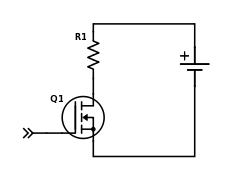
\includegraphics[scale=0.9]{Images/Dissipative_balancing.png}
		\caption{Schéma fonctionnel du balancement dissipatif}
		\label{fig:bal_dis}
	\end{minipage}
	\hfill
	\begin{minipage}{0.45\textwidth}
		\centering
		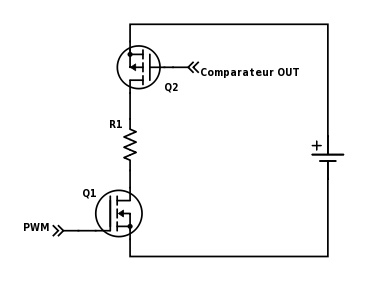
\includegraphics[scale=0.6]{Images/Dissipative_bal_comp.png}
		\caption{Schéma fonctionnel du balancement dissipatif avec redondance}
		\label{fig:bal_dis_comp}
	\end{minipage}	
\end{figure}

\subsubsection*{Balancement actif}
\paragraph*{}
Le balancement actif permet non seulement d'amener l'état de charge à 100\% mais aussi de l'amener à 0\%. Les modules qui ont une capacité supérieure peuvent transmettre l'énergie excédentaire aux modules avec une plus petite capacité. L'utilisation de la batterie est ainsi optimisée. Plusieurs topologies existent pour transférer l'énergie tel que des capacitances commutées, deux matrices qui connectent deux différents modules sur un convertisseur DC-DC, l'utilisation d'une inductance couplée pour faire un "Flyback" et plusieurs autres variantes. 

\paragraph*{}
L'utilisation d'un convertisseur DC-DC "Flyback", avec le primaire aux bornes de chaque module et le secondaire aux bornes de la batterie, est la topologie qui s'intègre le mieux pour son nombre de composantes limitées et sa simplicité d'utilisation. Le balancement actif est surtout utilisé pour des batteries qui ont des modules avec des performances très inégales et/ou des batterie qui ont une très grande durée de vie. Cette solution est plus robuste, puisqu'il suffit d'un fusible en série avec le bobinage primaire pour protéger la batterie d'une défaillance du MOSFET. Le courant de balancement peut aussi être beaucoup plus élevé étant donné qu'il n'y a pas beaucoup de perte.

\subsubsection*{Choix final}
\paragraph*{}
Le balancement dissipatif est la stratégie qui concorde le mieux aux besoins d'Éclipse X. La grosseur des transformateurs, l'ajout des fils pour connecter les bobinages secondaires, le manque de temps pour implémenter la solution et le faible gain de performance du balancement actif rendent cette solution impossible à utiliser pour le projet. La batterie d'Éclipse à seulement une durée de vie utile de 4 semaines en plus d'être construite avec des modules caractérisés qui ont des performances très semblables. Le balancement actif n'a pas de grande valeur ajoutée par rapport au balancement dissipatif.



